\subsection{Module 6: Theo dõi tình trạng đặt phòng cho chủ nhà}
\begin{figure}[!h]
	\centering
	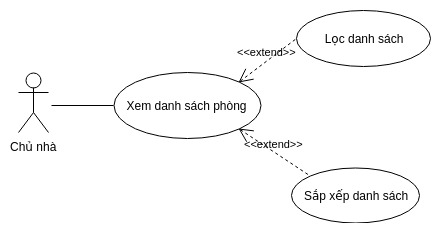
\includegraphics[width=\textwidth]{parts/Cuong/images/module5a.jpg}
	\caption{Lược đồ use case của module 5a: Theo dõi tình trạng đặt phòng cho chủ nhà}
\end{figure}

\subsubsection{User stories}
\begin{itemize}
    \item Chủ nhà có thể xem thông tin đặt phòng của các phòng mình đăng ký để biết một phòng đã có người đăng ký thành công, đăng ký nhưng chưa thanh toán, đang có người ở, hoặc đang trống.
    \item Chủ nhà có thể xem toàn bộ các phòng hoặc chỉ xem các phòng đã đăng ký thành công, hoặc các trạng thái khác đã đề cập ở trên.
    \item Chủ nhà có thể sắp xếp danh sách hiện tại theo một trường nào đó trong các trường được hiển thị.
\end{itemize}

% ########################################################
\subsubsection{Các use case chi tiết}
\subsubsubsection{Usercase 1: Xem danh sách phòng}
\begin{usecase}
    \usecasename{Xem danh sách phòng}
	\actor{Chủ nhà}
	\describe{Chủ nhà xem danh sách các phòng mình sở hiển thị}
	\creators{Văn Tiến Cường}{Văn Tiến Cường}
	\datecreated{22/03/2019}{30/03/2019}
	\precond{Chủ nhà đã đăng nhập thành công}
	\postcond{Hiện danh sách các phòng đã được đặt}
	
	\normalflow
	\begin{enumerate}
		\item Chủ nhà chọn mục \textbf{Danh sách phòng}.
        \item Hệ thống hiển thị danh sách đặt phòng.
	\end{enumerate} \\ \hline
	
	\noalternative
	\noexception
\end{usecase}

\subsubsubsection{Usercase 2: Lọc danh sách phòng}
\begin{usecase}
    \usecasename{Lọc danh sách phòng}
	\actor{Chủ nhà}
	\describe{Chủ nhà lọc danh sách phòng theo tình trạng đặt phòng}
	\creators{Văn Tiến Cường}{Văn Tiến Cường}
	\datecreated{30/03/2019}{30/03/2019}
	\precond{Chủ nhà đang xem danh sách phòng}
	\postcond{Hiện danh sách các phòng thoả điều kiện lọc}
	
	\normalflow
	\begin{enumerate}
		\item Chủ nhà chọn mục \textbf{Bộ lọc}.
        \item Hệ thống hiện thị các lựa chọn bộ lọc: \textbf{Đăng ký thành công}, \textbf{Chờ thanh toán}, \textbf{Đang ở}, \textbf{Phòng trống}.
        \item Người dùng chọn một trong các lựa chọn.
        \item Hệ thống lọc và hiển thị danh sách phòng phù hợp.
	\end{enumerate} \\ \hline
	
	\noalternative
	
	\exception
	\begin{itemize} 
		\alt{3a} Người dùng không chọn mục nào. Hệ thống sẽ hiển thị danh sách ban đầu.
	\end{itemize} \\ \hline 
\end{usecase}

\subsubsubsection{Usercase 3: Sắp xếp danh sách phòng}
\begin{usecase}
    \usecasename{Sắp xếp danh sách phòng}
	\actor{Chủ nhà}
	\describe{Chủ nhà sắp xếp danh sách phòng hiện tại theo một trường nào đó}
	\creators{Văn Tiến Cường}{Văn Tiến Cường}
	\datecreated{30/03/2019}{30/03/2019}
	\precond{Chủ nhà đang xem danh sách phòng}
	\postcond{Hiện danh sách các phòng thoả điều kiện lọc}
	
	\normalflow
	\begin{enumerate}
		\item Chủ nhà chọn mục \textbf{Sắp xếp theo}.
        \item Hệ thống hiện thị các lựa chọn sắp xếp: \textbf{Tên khách thuê}, \textbf{Ngày đến}, \textbf{Ngày đi}.
        \item Người dùng chọn một trong các lựa chọn.
        \item Hệ thống hiển thị danh sách phòng đã được sắp xếp.
	\end{enumerate} \\ \hline
	
	\noalternative
	
	\exception
	\begin{itemize} 
		\alt{3a} Người dùng không chọn mục nào. Hệ thống sẽ hiển thị danh sách ban đầu.
	\end{itemize} \\ \hline 
\end{usecase}